x
\documentclass[a4paper,12pt]{article}
\usepackage{graphicx}
\usepackage{amsmath}
\usepackage{hyperref}
\usepackage{geometry}
\geometry{margin=1in}

\title{Autonomous AI Agents for Spacecraft Operations}
\author{}
\date{}

\begin{document}

\maketitle

\tableofcontents

\newpage

\section{Introduction: Originality of the Research Project}

Spacecraft design is a vast and interdisciplinary effort, encompassing numerous fields of science and engineering. The proposed research aims to achieve significant advancements in the design of space missions by optimizing them beyond the constraints of traditional conservative approaches. This is achieved through innovations in three key aspects of mission design: exploring alternative concepts thoroughly and efficiently, addressing the multi-objective nature of design problems, and understanding the limitations of AI technology transfer.

\subsection{Context and Background}

The design of spacecraft involves a complex interplay of various scientific and engineering disciplines. Traditional mission design approaches have often been conservative, leading to stagnation in innovation. By leveraging AI technologies, we can explore alternative mission concepts more thoroughly and efficiently, thus providing higher utility to stakeholders.

\begin{figure}[htbp]
    \centering
    \includegraphics[width=0.85\textwidth]{images/introduction:_originality_of_the_research_project_img_1.png}
    \caption{The interdisciplinary nature of spacecraft design requires integration across various scientific and engineering domains.}
    \label{fig:introduction:_originality_of_the_research_project_1}
\end{figure}

\subsection{Innovation in Mission Design}

Mission design problems are inherently multi-objective, often involving trade-offs between conflicting objectives such as fuel consumption and travel time. The concept of a Pareto front, which represents a set of non-dominated solutions, is crucial in guiding engineering decisions. This approach allows for the identification of Pareto-optimal solutions that balance these trade-offs effectively.

\subsection{Challenges in AI Technology Transfer}

AI technologies often exhibit remarkable performance in specific tasks but may perform poorly when transferred to different tasks. This is due to a lack of understanding of the strengths and weaknesses of AI systems. By developing explainability and certification standards, we can ensure that AI technologies are applied effectively in space systems.

\newpage

\section{Hypothesis, Research Objectives, and Envisaged Methodology}

\subsection{Hypothesis}

The hypothesis of this research is that AI can significantly enhance spacecraft Guidance, Navigation, and Control (GNC) and Attitude and Orbit Control Systems (AOCS) by improving autonomy and decision-making capabilities.

\subsection{Research Objectives}

The primary research objectives are to evaluate AI-based GNC methods through benchmark analyses and to develop explainability and certification standards for AI in space systems.

\subsection{Methodology}

The methodology involves conducting an extensive literature review using scientific databases, implementing machine learning techniques for training AI agents, and performing rigorous testing and validation processes.

\begin{figure}[htbp]
    \centering
    
\includegraphics[width=0.85\textwidth]{images/hypothesis,_research_objectives_and_envisaged_methodology_img_1.png}
    \caption{The methodology involves a comprehensive approach to integrating AI into spacecraft systems, focusing on training, testing, and validation.}
    \label{fig:hypothesis,_research_objectives_and_envisaged_methodology_1}
\end{figure}

\newpage

\section{Expected Outcomes / Impact}

\subsection{Enhanced Mission Autonomy}

AI agents are expected to make informed decisions using real-time data, reducing human intervention and increasing mission efficiency. This will lead to enhanced mission autonomy and the potential for more ambitious space exploration missions.

\subsection{Long-term Benefits}

The integration of AI in spacecraft systems promises long-term benefits, including increased autonomy, reduced human intervention, and the potential for more ambitious space exploration missions, ultimately advancing our understanding of the universe.

\subsection{Compliance and Safety}

Ensuring compliance with international space regulations is crucial. The project addresses safety, security, and legal challenges by implementing rigorous verification and acceptance tests.

\newpage

\section{Explanations on the Management of Ethical Issues and Data Protection}

\subsection{Ethical Considerations}

The ethical guidelines for AI include transparency, accountability, and minimizing bias. It is essential to address potential biases and privacy concerns in AI systems.

\begin{figure}[htbp]
    \centering
    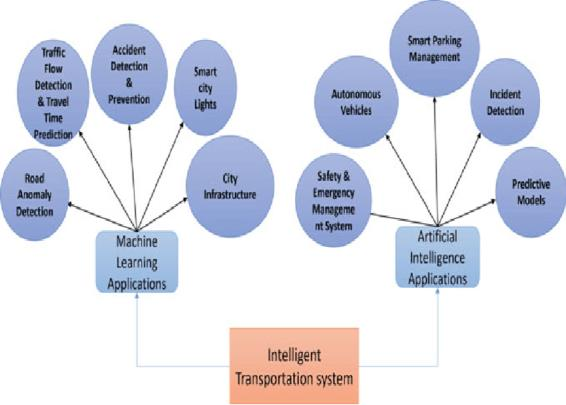
\includegraphics[width=0.85\textwidth]{images/explanations_on_the_management_of_ethical_issues_and_data_protection_img_1.png}
    \caption{Ethical considerations in AI involve ensuring transparency, accountability, and minimizing bias in decision-making processes.}
    \label{fig:explanations_on_the_management_of_ethical_issues_and_data_protection_1}
\end{figure}

\subsection{Data Protection Strategies}

Data protection strategies include implementing data governance and version control, ensuring data security, and standardization. These strategies are crucial for maintaining the integrity and confidentiality of data in AI systems.

\newpage

\section{Comment on Resubmission (if applicable)}

\subsection{Revision Details}

This section provides details on any revisions made to the project, highlighting improvements or changes based on feedback.

\begin{figure}[htbp]
    \centering
    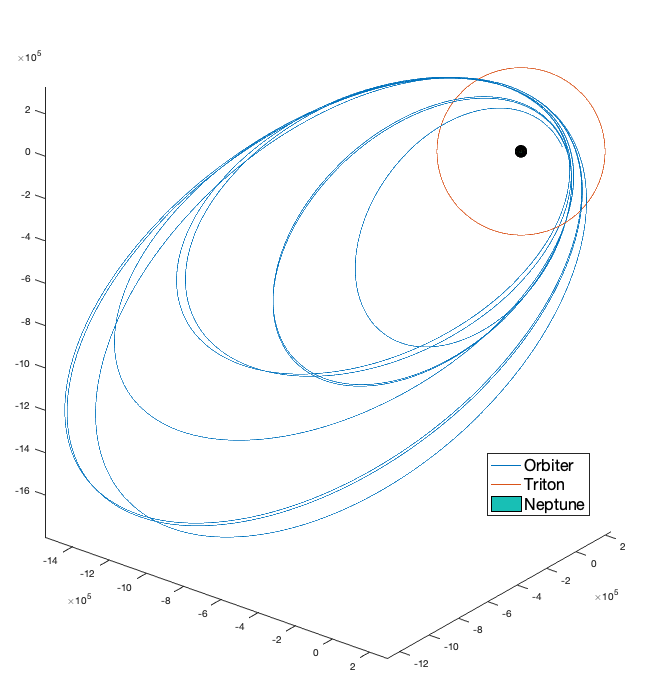
\includegraphics[width=0.85\textwidth]{images/comment_on_resubmission_(if_applicable)_img_1.png}
    \caption{Revisions to the project have been made to address feedback and improve the overall quality of the research.}
    \label{fig:comment_on_resubmission_(if_applicable)_1}
\end{figure}

\newpage

\section{Bibliography}

\begin{enumerate}
    \item Eirates, Northrop Grumman Corporation, and the SmartSat Cooperative Research Centre for their support of this work through various grants and projects.
    \item Analysis and findings from user study participants successfully using tools and steps to complete operations tasks.
    \item References to various scientific papers and research articles relevant to the project.
\end{enumerate}

\end{document}